\section{Annexes}
\appendix
\makeatletter
\def\@seccntformat#1{Annexe~\csname the#1\endcsname:\quad}
\makeatother

\section{Revue des méthodes explicatives}
\begin{figure}[h]
\centering
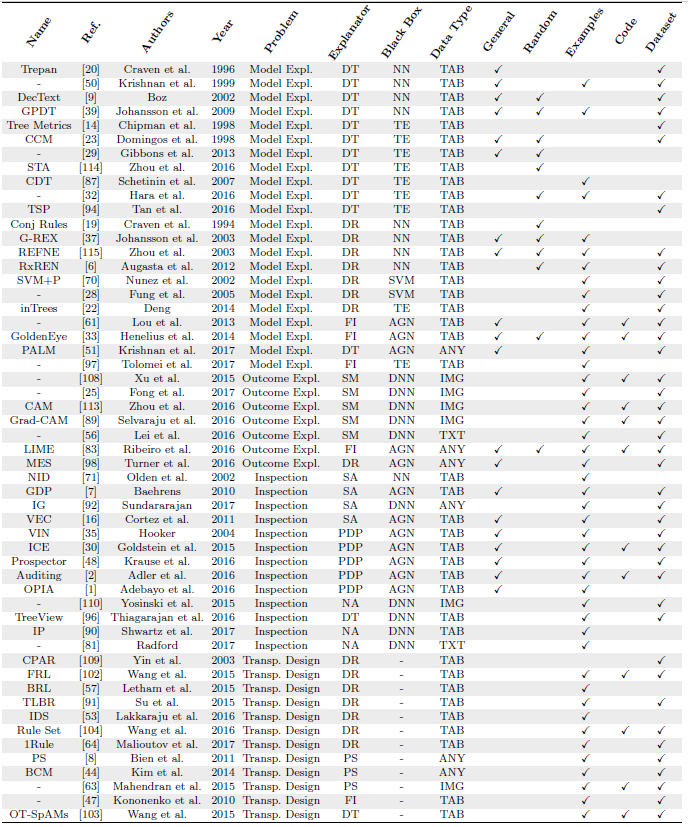
\includegraphics[scale=1.01]{src_img/tabSummary.PNG}
\caption{Tableau résumant l'ensemble des méthodes expliquant les boites noires présent dans la littérature. Description en annexe 2. Tiré de \cite{surveyExplaining}}
\label{tabSummary}
\end{figure}

\newpage

\section{Description des méthodes explicatives}
\begin{figure}[h]
\centering
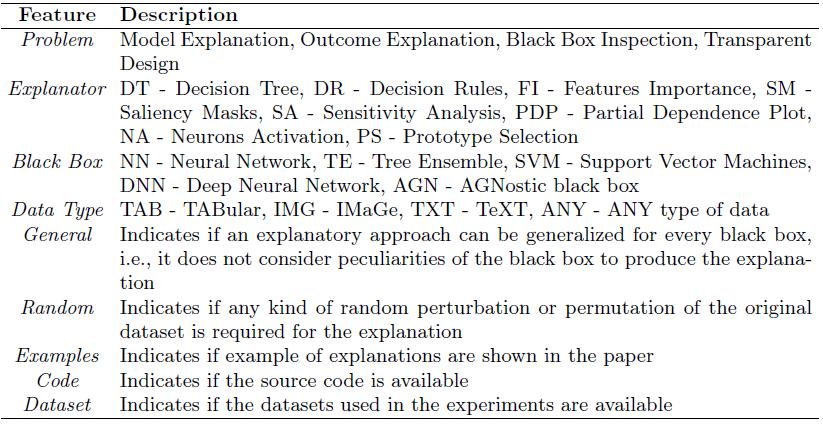
\includegraphics[scale=1.01]{src_img/descSummary.PNG}
\caption{Description du tableau présent en annexe 1. Tiré de \cite{surveyExplaining}}
\label{descSummary}
\end{figure}